% arara: xelatex: { shell: yes, synctex: yes }
\RequirePackage[l2tabu, orthodox]{nag}
\documentclass{article}

% -- Texto e codificação
\usepackage{anyfontsize}
\usepackage{pdflscape}



% -- Símbolos extra
\usepackage{amssymb}
\usepackage{textcomp}
\usepackage{gensymb}
\usepackage{cancel}

% -- Redefine margins
\geometry{top = 1cm}

% -- Bibliografia
\usepackage[
	backend = biber,
	style = alphabetic,
	sorting = ynt,
	%alldates=iso
	]{biblatex}
\usepackage{fvextra}
\usepackage{csquotes}

% --  Definições de imagens
\graphicspath{{graphics/}}
\usepackage{caption}
\usepackage{subcaption}
\usepackage{afterpage}
\usepackage{tabularx}

% -- Desenhar circuitos elétricos e lógicos
\usepackage{tikz}
\usepackage{pgfplots}
\usepackage{circuitikz}
\usetikzlibrary{arrows.meta,positioning,patterns,graphs}
\pgfplotsset{compat=1.15}
\pgfplotsset{table/search path = {data}}
\pgfplotsset{/pgf/number format/use comma,}

% -- Integrar código fonte
\usepackage{minted}
\usepackage{verbatim}
\usepackage{algorithm}
\usepackage{algpseudocode}

% -- Tabelas
\usepackage{booktabs}
\usepackage{makecell}

% -- Misc
\usepackage[disable]{todonotes}

% -- Funções matemáticas extra
\usepackage{siunitx}
\sisetup{
  math-ohm=\Omega,
  text-ohm=\ensuremath{\Omega},
}
\usepackage{circuitikz}
\usetikzlibrary{positioning}

\newcommand{\matr}[1]{\mathbf{#1}}

\addbibresource{bibliography.bib}

\begin{document}

\begin{titlepage}

\begin{center}
	\vspace*{0.1\textheight}
	
\includegraphics[width = 0.4\linewidth, trim = {172.4pt 202.7pt 172.6pt 201.4pt}, clip]{IST_A_CMYK_POS}
	
	\vspace*{0.1\textheight}
	{\huge\bfseries Real-Time Cooperative Decentralized Control of a Smart Office Illumination System}
	
	\vspace*{0.03\textheight}
	{\Large Distributed Real-Time Control Systems Final Project}
	
	\vspace*{43.5mm}
	{\Large \begin{tabular}{l r} Daniel de Schiffart & \texttt{81479} \\ João Gonçalves & \texttt{81040} \\ Francisco Castro & \texttt{78655}\end{tabular}}
	
	\vspace{\fill}
	{\large Distributed Real-Time Control Systems}
	
	\vspace*{0.01\textheight}
	{\Large Master's Degree in Aerospace Engineering}
	
	\vspace*{0.01\textheight}
	{\large Instituto Superior Técnico}
\end{center}

\end{titlepage}
\setcounter{page}{1}

{\hypersetup{linkcolor = black} \tableofcontents}

\section{Introdução}

\todo[inline]{Mencionar que toda a implementação é feita para 2 nodes, apesar de ser tudo extensível, blah blah}

\section{Raspbian Startup}
\begin{enumerate}
	\item Open console
	\item \texttt{sudo ifconfig enp2s0f0 10.0.0.2 netmask 255.255.255.0}
	\item Configure by hand on Ubuntu wired connection settings
	\begin{enumerate}
		\item Details -> Disable \textit{Connect Automatically}
		\item IPv4 -> \textit{IPv4 Method} to \textit{Manual}
		\item Set address to \texttt{10.0.0.2} and gateway to \texttt{255.255.255.0}
	\end{enumerate}
	\item Run \texttt{ssh pi\@10.0.0.1} and use \texttt{raspberry} as password
\end{enumerate}

\paragraph{Importante} Antes de desligar o Raspberry Pi, correr \texttt{sudo shutdown -h now} para evitar corrupção do sistema operativo.


\section{Illumination system calibration}

\subsection{Principles of the calibration procedure}

The illuminance at each desk follows the model
\begin{align}
  L &= K \mathbf{d} + \mathbf{o} \nonumber \\ 
  \left[\begin{array}{c} l_{1}\\ l_{2} \end{array}\right] &=
  \left[\begin{array}{cc}
	k_{11} & k_{12}\\
	k_{21} & k_{22}
  \end{array}\right]
  \left[\begin{array}{c} d_{1}\\ d_{2}\end{array}\right]+
  \left[\begin{array}{c} o_{1}\\ o_{2} \end{array}\right],
  \label{eq:model}
\end{align}
where $l_i$, $d_i$ and $o_i$ are the illuminance, LED power (in percentage) and background illuminance at desk $i$, respectively. The purpose of the calibration is to find the values for $k_{ij}$ and $o_i$ for a given office layout.

The calibration is performed by turning the lumiaires synchronously and taking measurements. One node takes initiative and sends a message to trigger the process. First, both LEDs are switched off and $o_i$ is measured.
Then, node 2 turns on its LED, measures the resulting illuminance and computes $k_{22}$, and sends the illuminance to node 1. Receiving this value, node 1 can also measure its illuminance and compute $k_{21}$. The operation inverts and $k_{12}$ and $k_{11}$ are determined. In the end, nodes share the results.

\subsection{Implementation detais}

The previous procedure is implemented as its own module, with a special communication protocol. The flow chart in figure \ref{fig:cal} illustrates messages sent and summarizes the finite-state machine.
Between changing the LED state and taking measurements, the nodes must sleep, to guarantee that the measurement is taken in steady state. For this, they were set to sleep for a lenght of time 10 times the value of the system time constant, $10 \times \SI{5}{\milli \second} = \SI{50}{\milli \second}$. 

\begin{figure}[ht]
  \centering
  \missingfigure{Diagrama da maquina de estados, em tikz}
  \caption{Calibration finite-state machine, with communication events.}
  \label{fig:cal}
\end{figure}

It also should be noted that internally, the nodes are not distinguishable as 1 and 2. Each considers itself node 1 and the peer as 2, so the representation of the coupling matrix $K$ is transposed by both diagonals, and identically $o_1$ and $o_2$ are swapped.

\section{Optimização do Sistema Distribuído}

\begin{gather*}
	u^* = \textrm{argmin}\,J(x, \mu) \\
	l_i = \sum^n_{j=1} d_j k_{ij} + o_i \geq L_i, \qquad 0 \leq d_i \leq 100, \quad \forall i \\
	\matr{l} = \matr{K}\matr{d} + \matr{o} \geq \matr{L}, \qquad 0 \leq d \leq 100
\end{gather*}
Se as condições aqui listadas não forem cumpridas, o problema é declarado \textit{unfeasible}. A função de custo é
\begin{gather*}
	f(d) = c_1d_1 + c_2d_2 + \ldots + c_nd_n = \matr{C}^T\matr{d}
\end{gather*}
onde $\matr{c}$ é o vetor dos custos de energia.

Ver os cantos do domínio admissível e saber o ponto com menor custo. Assim, obtém-se $(d_1,d_2)$. Mais à frente adicionamos maximização de longevidade de lâmpadas.
\begin{figure}[ht]
	\centering
	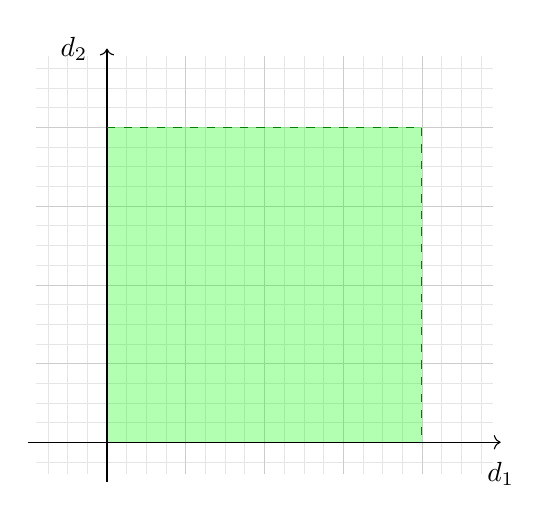
\begin{tikzpicture}
		\coordinate (axis) at (0,0);
		\node at (0,5) [label={180:$d_2$}] {};
		\node at (5,0) [label={-90:$d_1$}] {};
		\draw [step=0.25,draw=black!10!white,very thin] (-0.9,-0.4) grid (4.9,4.9);
		\draw [step=1,draw=black!20!white,very thin] (-0.9,-0.4) grid (4.9,4.9);
		\fill [fill=green,opacity=0.3] (0,0) -- (0,4) -- (4,4) -- (4,0) -- cycle;
		\draw [->] (axis) ++(0,-0.5) -- (0,5);
		\draw [->] (axis) ++(-1,0) -- (5,0);
		\draw [dashed,color={green!50!black}] (axis) (0,4) -- (4,4) -- (4,0);
	\end{tikzpicture}
\end{figure}

\appendix
\section{Esquemas}

\begin{tikzpicture}
	\tikzstyle{arduino} = [draw,minimum height=80,inner sep=30];
	\tikzstyle{wire} = [];
	\node at (0,0) (ard1) [arduino] {\Large Arduino 1};
	\node (ard2) [right=4cm of ard1,arduino] {\Large Arduino 2};
	\node (rpi) [above=2cm of ard2,arduino] {\Large Raspberry Pi};
	\path (ard1.north east) to node (ard1_scl) [auto, swap, align=right] {\ttfamily SCL} ++(0,-3);
	\path (ard1.north east) to node (ard1_sda) [auto, swap, align=right] {\ttfamily SDA} ++(0,-4);
	\path (ard1.north east) to node (ard1_gnd) [auto, swap, align=right] {\ttfamily GND} ++(0,-5);
	\path (ard2.north west) to node (ard2_scl) [auto, align=left] {\ttfamily SCL} ++(0,-3);
	\path (ard2.north west) to node (ard2_sda) [auto, align=left] {\ttfamily SDA} ++(0,-4);
	\path (ard2.north west) to node (ard2_gnd) [auto, align=left] {\ttfamily GND} ++(0,-5);
	\path (rpi.north west) to node (rpi_19) [auto, align=left] {\ttfamily 19} ++(0,-3);
	\path (rpi.north west) to node (rpi_18) [auto, align=left] {\ttfamily 18} ++(0,-4);
	\path (rpi.north west) to node (rpi_gnd) [auto, align=left] {\ttfamily GND} ++(0,-5);
	\draw (ard1_scl) -- (ard2_scl) (ard1_sda) -- (ard2_sda) (ard1_gnd) -- (ard2_gnd);
	\path (ard1_scl) ++(1.7,0) coordinate (coord1);
	\path (ard1_sda) ++(2.4,0) coordinate (coord2);
	\path (ard1_gnd) ++(3.1,0) coordinate (coord3);
	\draw (coord1) to [short,*-,R] (coord1 |- rpi_19) to [short,-] (rpi_19.west);
	\draw (coord2) to [short,*-,R] (coord2 |- rpi_18) to [short,-] (rpi_18.west);
	\draw (coord3) to [short,*-] (coord3 |- rpi_gnd) to [short,-] (rpi_gnd.west);
\end{tikzpicture}

\pagebreak
\printbibliography


\listoftodos
\end{document}
